%% Author: Daniel Kaplan
%% Subject: Distributions (comparing different displays)




\providecommand{\HCode}[1]{#1} % dummy, just in case it's PDFlatex
\HCode{<link rel="stylesheet" href="fixSweave.css" type="text/css"
  media="screen" />}
\HCode{<link rel="stylesheet" href="http://dl.dropbox.com/u/5098197/Math135/RGuide/fixSweave.css" type="text/css"
 media="screen" />}

The boxplots below are all made from exactly the same data.  One of
them is made correctly, according to the ``1.5 IQR'' convention for
drawing the whiskers.  The others are drawn differently.


\centerline{\begin{tabular}{cccc}
{\bf Plot 1} & {\bf Plot 2} & {\bf Plot 3} & {\bf Plot 4}\\
 & & \\
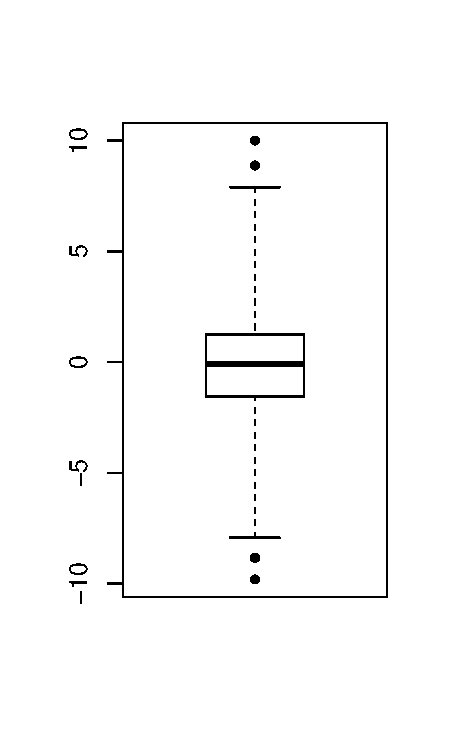
\includegraphics[width=.8in,trim=35 30 25 30]{Figures/B101-b1}
&
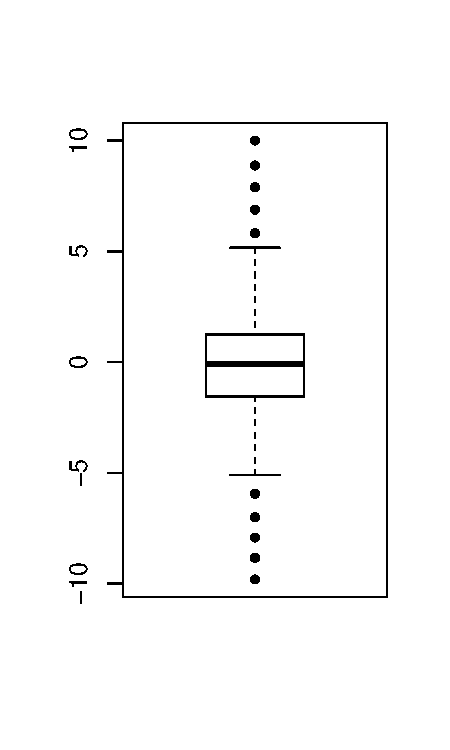
\includegraphics[width=.8in,trim=35 30 25 30]{Figures/B101-b2}
&
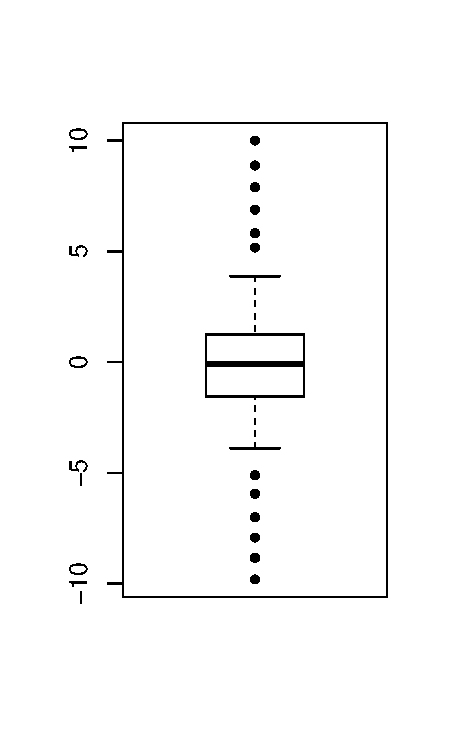
\includegraphics[width=.8in,trim=35 30 25 30]{Figures/B101-b3}
&
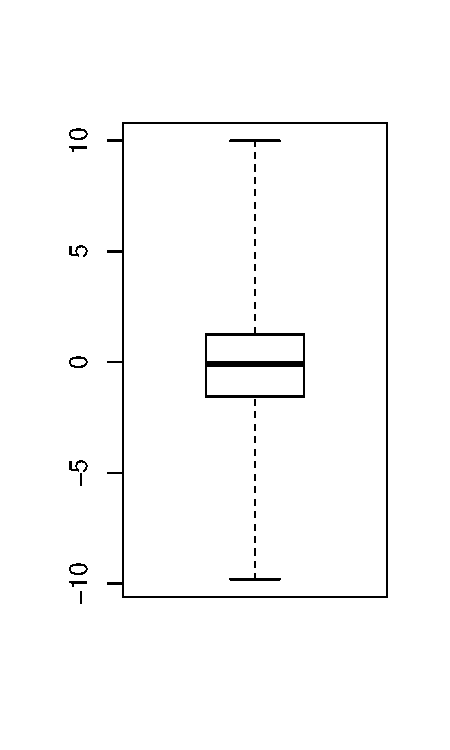
\includegraphics[width=.8in,trim=35 30 25 30]{Figures/B101-b4}
\\
\end{tabular}}

\begin{itemize}
\item Which of the plots is correct? \SelectSetHoriz{2}{1,2,3,4}
\end{itemize}

\begin{AnswerText}
The height of the box gives the IQR.  If there are outliers, the whisker length should be 1.5
times the IQR.  So look for the plot that has a whisker length
somewhat taller than the box itself.
\end{AnswerText}

